\section{Въведение}
Капилярните мостове са резултат от минимизирането на повърхността на течност
,,разпъната`` между две твърди тела или течни повърхности с произволна форма.

Това е причината капилярните мостове още да се наричат и ,,капилярни връзки`` (capillary bonds),
тъй като те възникват най-често в практиката като течна връзка при опит за разделяне на две
твърди повърхности омокрени от течност между тях - напр. някои животни могат да ,,залепват`` към
стени, като ,,инжектират`` омокряща течност между \cite{Persson_2007} крайниците си и стената.
Важно значение имат и за агрерирането на частиците в колоидни разтвори, АФМ, омокрянето на прахове и др.

Историята на изследванията им започва с дефинираната от Лагранж задача за мимимизираща повърхност
при дадени граници. Проблемът за намирането на тази повърхност обаче е известен в литературата
като ,,задачата на Плато``, който експерментира със сапунени филми с фиксирани граници.
Той идентифицира седем тела с постоянна гаусова кривина, които описват профила на капилярните мостове:
\begin{enumerate*}
    \item Нодоид с ,,шия``
    \item Катеноид
    \item Ундулоид с ,,шия``
    \item Цилиндър
    \item Ундулоид с ,,гърбица``
    \item Сфера
    \item Нодоид с ,,гърбица``.
\end{enumerate*}
За 1. до 5. капилярните сили трябва да са на привличане, за сфера да са 0, а за 7. да са на
отблъскване. При \cite{Kralchevsky}
Когато границите са тороидни (,,кръгли``), то при сапунените филми се получава профил на катеноид \autoref{fig:soap_cath}.
\begin{figure}[h]
    \centering
    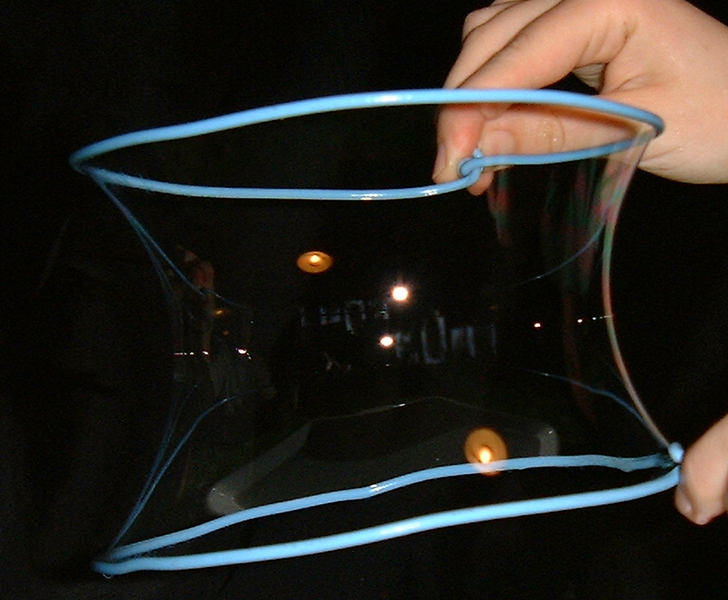
\includegraphics[width=0.4\linewidth]{cathenoid_soap.png}
    \caption{Сапунен мехур с тороидни граници (телчетата).\cite{Soap_cathenoid}}
    \label{fig:soap_cath}
\end{figure}

Най-простите повърхности, между които може да се формира 